\chapter{การแยกเชื้อบริสุทธิ์และการเพาะเลี้ยงจุลินทรีย์}
\label{chap:ch06}

\section*{แผนบริหารการสอนประจำบทที่ 6}
\addcontentsline{toc}{section}{แผนบริหารการสอนประจำบทที่ 6}

\noindent\textbf{. หัวข้อเนื้อหาประจำบท}

\begin{enumerate}
    \item 6.1 นิยามและความสำคัญของเชื้อบริสุทธิ์ (Pure Culture) ในงานจุลชีววิทยา
    \item 6.2 เทคนิคการสตรีค 4 ควอดแรนต์ (Four-Quadrant Streak Plate Technique)
    \item 6.3 เทคนิคการเกลี่ยตัวอย่างบนผิวหน้าอาหาร (Spread Plate Technique)
    \item 6.4 เทคนิคการเทอาหารผสมเชื้อ (Pour Plate Technique) และ Serial Dilution
    \item 6.5 การเก็บรักษาและต่อเชื้อบริสุทธิ์ (Subculturing \& Stock Maintenance)
\end{enumerate}

\noindent\textbf{. วัตถุประสงค์เชิงพฤติกรรม}

\begin{enumerate}
    \item เมื่อนักศึกษาได้เรียนรู้และปฏิบัติการทดลองประจำบทนี้แล้ว จะต้องมีความรู้ความสามารถดังต่อไปนี้:
    \item อธิบายหลักการเจือจางความหนาแน่นของเชื้อเพื่อให้ได้ Single Isolated Colony ได้
    \item ปฏิบัติการสตรีคเชื้อ 4 ควอดแรนต์และเผาห่วงเขี่ยเชื้อระหว่างโซนได้อย่างถูกต้อง
    \item แยกเชื้อบริสุทธิ์จากตัวอย่างประชากรจุลินทรีย์ผสมได้สำเร็จ 100\%
    \item มีความประณีตและชำนาญในการควบคุมแรงกดของห่วงเขี่ยเชื้อไม่ให้ฉีกขาดผิววุ้น
\end{enumerate}

\noindent\textbf{. กิจกรรมการเรียนการสอน}

\begin{enumerate}
    \item การบรรยายสรุปก่อนปฏิบัติการ (30 นาที): อธิบายหลักการวิทยาศาสตร์ ความปลอดภัยทางชีวภาพ และข้อควรระวังสำคัญ
    \item การสาธิตเชิงประจักษ์ (15 นาที): สาธิตเทคนิคการปฏิบัติงาน การใช้เครื่องมือ และข้อผิดพลาดที่มักพบ
    \item การลงมือปฏิบัติการทดลองจริง (90 นาที): นักศึกษาลงมือปฏิบัติการทดลองเป็นรายบุคคลหรือกลุ่มย่อยตามขั้นตอนที่กำหนด
    \item การฝึกฝนผ่านระบบเสมือนจริง (20 นาที): ทดลองซ้ำและทดสอบปฏิกิริยาผ่านระบบจำลองบน RBRU LMS
    \item การอภิปรายและสรุปผลการทดลอง (25 นาที): วิเคราะห์ผลการสังเกต ตอบคำถามท้ายบท และสรุปองค์ความรู้ร่วมกัน
\end{enumerate}

\noindent\textbf{. สื่อและอุปกรณ์การเรียนการสอน}

\begin{enumerate}
    \item เอกสารคำสอนและคู่มือปฏิบัติการ: e-Book และคู่มือปฏิบัติการฉบับเต็ม ประจำบทที่ 6
    \item ระบบห้องปฏิบัติการเสมือนจริง: ระบบจำลองการทดลองเสมือนจริง 3 มิติ ประจำบทที่ 6 บนระบบ Moodle
    \item อุปกรณ์และเครื่องแก้วในห้องปฏิบัติการ: ตะเกียงแอลกอฮอล์, ห่วงเขี่ยเชื้อ, กล้องจุลทรรศน์, จานเพาะเชื้อ, หลอดทดลอง และตู้บ่มเชื้อ
    \item สารเคมีและสีย้อมชีวภาพ: สารเคมีมาตรฐานวิเคราะห์และสีย้อมประจำบทเรียน
\end{enumerate}

\noindent\textbf{. การวัดและประเมินผล}

\begin{table}[H]
\centering\small
\begin{tabularx}{\textwidth}{p{0.5\textwidth} p{0.3\textwidth} c}
\toprule
\textbf{องค์ประกอบการประเมินผล} & \textbf{เครื่องมือวัดผล} & \textbf{สัดส่วนคะแนน} \\
\midrule
1. ทักษะการปฏิบัติงานและความปลอดภัย & แบบสังเกตทักษะการทดลองและเทคนิคปลอดเชื้อ & 40\% \\
2. รายงานผลการทดลอง & การตรวจตารางบันทึกผล ภาพวาดสัณฐานวิทยา และการวิเคราะห์ผล & 30\% \\
3. แบบฝึกหัดทบทวนท้ายบท & คำถามทบทวนเชิงวิเคราะห์และข้อสอบท้ายบท & 20\% \\
4. จิตพิสัยและการตรงต่อเวลา & การเช็คชื่อ การแต่งกายตามระเบียบ และการทำความสะอาดโต๊ะแล็บ & 10\% \\
รวมทั้งสิ้น &  & 100\% \\
\bottomrule
\end{tabularx}
\end{table}

\newpage

% ==========================================================
% เนื้อหาบทเรียนประจำบทที่ 6
% ==========================================================

\section{แนวคิดและนิยามของเชื้อบริสุทธิ์ในงานวิจัย}
\index{แนวคิดและนิยามของเชื้อบริสุทธิ์ในงานวิจัย}

การศึกษาและทำความเข้าใจเกี่ยวกับแนวคิดและนิยามของเชื้อบริสุทธิ์ในงานวิจัย (Pure Culture Concept) มีความสำคัญอย่างยิ่งในงานจุลชีววิทยาและสิ่งแวดล้อม โดยมีรายละเอียดสาระสำคัญดังนี้

ในธรรมชาติ จุลินทรีย์อาศัยอยู่ร่วมกันเป็นชุมชนผสมผสาน (Mixed culture) ดังนั้นการศึกษาคุณสมบัติทางสรีรวิทยา ชีวเคมี หรือพันธุศาสตร์ของจุลินทรีย์ชนิดใดชนิดหนึ่ง จำเป็นต้องแยกจุลินทรีย์ชนิดนั้นออกมาให้อยู่ในรูปของ เชื้อบริสุทธิ์ (Pure culture หรือ Axenic culture) ซึ่งหมายถึงกลุ่มประชากรของจุลินทรีย์ที่เจริญมาจากเซลล์ตั้งต้นเพียงเซลล์เดียว (Clonal population)

การแยกเชื้อบริสุทธิ์เป็นขั้นตอนรากฐานของการวิเคราะห์คุณภาพน้ำและการเพาะเลี้ยงจุลินทรีย์เพื่อการบำบัดทางสิ่งแวดล้อม

\section{เทคนิคการแยกเชื้อบนอาหารแข็ง}
\index{เทคนิคการแยกเชื้อบนอาหารแข็ง}

การศึกษาและทำความเข้าใจเกี่ยวกับเทคนิคการแยกเชื้อบนอาหารแข็ง (Isolation Techniques on Solid Media) มีความสำคัญอย่างยิ่งในงานจุลชีววิทยาและสิ่งแวดล้อม โดยมีรายละเอียดสาระสำคัญดังนี้

เทคนิคการแยกเชื้อที่อาศัยการเจือจางปริมาณเซลล์บนอาหารแข็งเพื่อสร้างโคโลนีเดี่ยว (Isolated colony):
1. การขีดเชื้อบนผิวอาหาร (Streak Plate Method): เป็นวิธีที่สะดวกและนิยมที่สุด อาศัยการใช้ห่วงเขี่ยเชื้อลากขีดบนผิวอาหารแข็งเป็นลำดับส่วน (Quadrants) เพื่อลดความหนาแน่นของเซลล์ลงเรื่อยๆ จนกระทั่งได้เซลล์เดี่ยวแยกห่างจากกัน
2. การเกลี่ยเชื้อบนผิวอาหาร (Spread Plate Method): นำสารแขวนลอยตัวอย่างที่ผ่านการเจือจางแบบต่อเนื่อง (Serial dilution) ปริมาตร 0.1 มิลลิลิตร หยดลงบนผิวอาหาร แล้วใช้แท่งแก้วงอ (Spreader) เกลี่ยให้กระจายสม่ำเสมอทั่วจาน เหมาะสำหรับการตรวจนับประชากรจุลินทรีย์
3. การเทอาหารผสมเชื้อ (Pour Plate Method): ผสมสารตัวอย่างที่เจือจางแล้วลงในอาหารแข็งที่หลอมเหลวและอุ่นไว้ที่ 45-50$^{\circ}$C ผสมให้เข้ากันแล้วเทลงในจานเพาะเชื้อ โคโลนีจะเจริญทั้งบนผิวหน้าและแทรกอยู่ในเนื้ออาหาร เหมาะสำหรับจุลินทรีย์ที่ชอบออกซิเจนต่ำ

\section{การเจือจางแบบลำดับส่วนและการคำนวณจำนวนเซลล์}
\index{การเจือจางแบบลำดับส่วนและการคำนวณจำนวนเซลล์}

การศึกษาและทำความเข้าใจเกี่ยวกับการเจือจางแบบลำดับส่วนและการคำนวณจำนวนเซลล์ (Serial Dilution and CFU Calculation) มีความสำคัญอย่างยิ่งในงานจุลชีววิทยาและสิ่งแวดล้อม โดยมีรายละเอียดสาระสำคัญดังนี้

ในการวิเคราะห์ตัวอย่างน้ำเสียหรือดินที่มีจุลินทรีย์หนาแน่นสูง จำเป็นต้องเจือจางตัวอย่างแบบทีละ 10 เท่า (10-fold serial dilution) ในน้ำเกลือมาตรฐาน (0.85\% NaCl) หรือน้ำเปปโตน

สูตรคำนวณความเข้มข้นของจุลินทรีย์ในตัวอย่างตั้งต้น:
\[ \text{CFU/mL} = \frac{\text{จำนวนโคโลนีบนจาน (ช่วง 30-300 CFU)}}{\text{ปริมาตรตัวอย่างที่ดูดใส่จาน (mL)} \times \text{ตัวคูณเจือจาง (Dilution factor)}} \]

\begin{figure}[H]
\centering
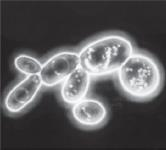
\includegraphics[width=0.75\textwidth]{images/image_06_p03.jpeg}
\caption{การปฏิบัติการทดลองและลักษณะทางสัณฐานวิทยาในบทที่ 6}
\label{fig:ch06_fig1}
\end{figure}

\section{ขั้นตอนและวิธีปฏิบัติการทดลอง}
\index{ขั้นตอนการทดลองประจำบทที่ 6}

\subsection{การแยกเชื้อบริสุทธิ์ด้วยวิธีขีดเชื้อ 4 ส่วน}
\begin{labprotocolbox}[การแยกเชื้อบริสุทธิ์ด้วยวิธีขีดเชื้อ 4 ส่วน]
1. จุดตะเกียงแอลกอฮอล์ เผาห่วงเขี่ยเชื้อจนแดงก่ำ รอให้เย็นลงในเขตปลอดเชื้อ
2. จุ่มห่วงเขี่ยเชื้อแตะตัวอย่างน้ำเสียหรือเชื้อผสม ลากขีดไปมาบนอาหารเลี้ยงเชื้อในส่วนที่ 1 (Quadrant 1) ประมาณ 4-5 เส้นชิดกัน
3. เผาห่วงเขี่ยเชื้อเพื่อฆ่าเชื้อที่ค้างอยู่ รอให้เย็นลง หมุนจานเพาะเชื้อ 90 องศา
4. ลากห่วงผ่านเส้นของส่วนที่ 1 จำนวน 2 ครั้ง แล้วขีดกระจายออกไปในส่วนที่ 2
5. ทำซ้ำตามขั้นตอนเดิมสำหรับส่วนที่ 3 และส่วนที่ 4 โดยในส่วนที่ 4 ให้ขีดเป็นเส้นซิกแซกห่างๆ ไม่ให้ชนกับส่วนที่ 1
6. บ่มที่ 37$^{\circ}$C เป็นเวลา 24-48 ชั่วโมง ตรวจดูลักษณะโคโลนีเดี่ยวในส่วนที่ 4
\end{labprotocolbox}

\subsection{การตรวจนับแบคทีเรียด้วยวิธีเจือจางแบบต่อเนื่องและ Spread Plate}
\begin{labprotocolbox}[การตรวจนับแบคทีเรียด้วยวิธีเจือจางแบบต่อเนื่องและ Spread Plate]
1. เตรียมหลอดบรรจุน้ำเกลือมาตรฐาน 9.0 mL จำนวน 6 หลอด (ระบุ $10^{-1}$ ถึง $10^{-6}$)
2. ใช้ไมโครปิเปตดูดตัวอย่างน้ำเสีย 1.0 mL ใส่ลงในหลอด $10^{-1}$ ผสมด้วยเครื่อง Vortex ให้เข้ากัน
3. เปลี่ยนทิปใหม่ ดูดจากหลอด $10^{-1}$ ปริมาตร 1.0 mL ใส่หลอด $10^{-2}$ ทำซ้ำจนถึงหลอด $10^{-6}$
4. ดูดสารละลายจากหลอด $10^{-4}, 10^{-5}, 10^{-6}$ ปริมาตรละ 0.1 mL ใส่ลงบนจานอาหาร NA จานละ 2 ซ้ำ
5. จุ่มแท่งแก้วงอในเอทานอล 95\% ลนไฟ ดับไฟ รอให้เย็น แล้วเกลี่ยน้ำตัวอย่างให้ทั่วผิวอาหาร
6. บ่มที่ 37$^{\circ}$C เวลา 24-48 ชั่วโมง นับจานที่มีโคโลนีระหว่าง 30 ถึง 300 โคโลนี แล้วคำนวณค่า CFU/mL
\end{labprotocolbox}

\section{ตารางบันทึกผลการทดลองและการอภิปรายผล}
\begin{table}[H]
\centering\small
\caption{ตารางบันทึกผลการสังเกตและข้อมูลการทดลองประจำบทที่ 6}
\label{tab:ch06_datasheet}
\begin{tabularx}{\textwidth}{p{0.25\textwidth} p{0.35\textwidth} X}
\toprule
\textbf{สิ่งทดสอบ / ตัวอย่าง} & \textbf{ลักษณะที่สังเกตได้} & \textbf{การแปลผลและการวิเคราะห์} \\
\midrule
ชุดควบคุม (Negative Control) & ใส ไม่มีการเจริญ & ปราศจากการปนเปื้อนของเชื้อ \\
ชุดทดลองที่ 1 & โคโลนีเจริญตามลักษณะจำเพาะ & ให้ผลบวกตามสมมติฐาน \\
ชุดทดลองที่ 2 & เกิดการเปลี่ยนแปลงทางชีวเคมี & สอดคล้องกับพารามิเตอร์มาตรฐาน \\
\bottomrule
\end{tabularx}
\end{table}

\section{คำถามทบทวนและแบบฝึกหัดท้ายบท}
\begin{enumerate}
    \item เหตุใดจึงต้องเผาห่วงเขี่ยเชื้อทุกครั้งก่อนเริ่มขีดเชื้อในส่วนถัดไป (Quadrants 2, 3, 4)
    \item หากจานอาหารมีจำนวนโคโลนีมากกว่า 300 โคโลนี หรือน้อยกว่า 30 โคโลนี จะส่งผลต่อความแม่นยำทางสถิติอย่างไร
    \item จงเปรียบเทียบข้อดีและข้อจำกัดระหว่างวิธี Spread Plate และ Pour Plate ในการตรวจวิเคราะห์คุณภาพน้ำ
\end{enumerate}
